\section{Vercel}

El despliegue de la aplicación se realiza utilizando \textit{Vercel}, una plataforma de hosting orientada a aplicaciones frontend y serverless. La principal razón por la que se ha seleccionado esta plataforma, de entre las muchas opciones, es porque \textit{Vercel} es la empresa desarrolladora del framework \textit{Next.js}. Con esto se asegura una integración completa y se simplifica significativamente el proceso de despliegue.

También ha sido importante el hecho de que la infraestructura de \textit{Vercel} se apoya en servicios como \textit{Amazon Web Services} y \textit{Cloudflare} \cite{vercelInfrastructure2023}, entidades muy conocidas y confiadas, que proporcionan características de seguridad, disponibilidad y alto rendimiento. Sobre ellas, \textit{Vercel} ofrece una interfaz muy cómoda para manejar los despliegues, además de un sistema de despliegue continuo muy accesible.

\section{Límites y Características}

Para este proyecto, el plan gratuito \textbf{Hobby} de \textit{Vercel} ofrece unas características suficientes, ya que está dirigido a proyectos personales o de pequeña escala. En la tabla \ref{tab:vercel_plan_hobby}, se listan los principales límites de los recursos disponibles:

\begin{table}[htbp]
    \centering
    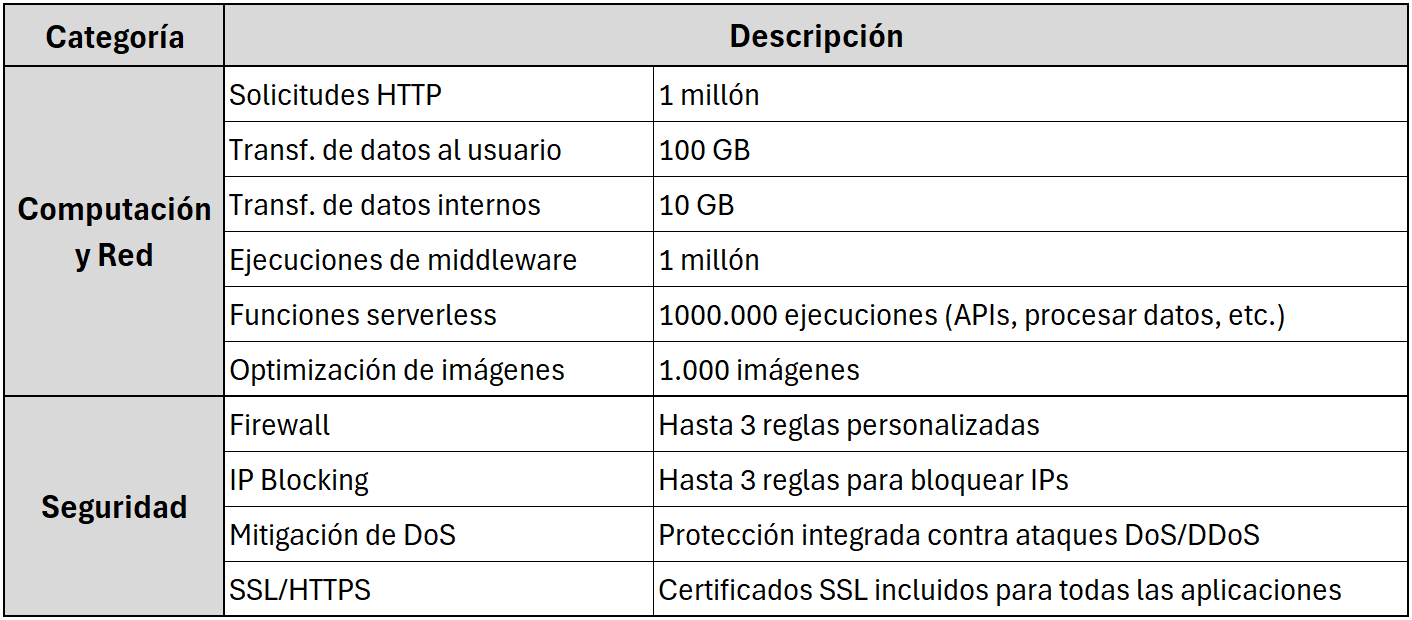
\includegraphics[width=0.9\textwidth]{figures/despliegue/vercel_plan_hobby.png}
    \captionsetup{skip=10pt}
    \caption{Límites y características por mes del plan \textit{Hobby} de \textit{Vercel}.}
    \label{tab:vercel_plan_hobby}
\end{table}

\section{Proceso de Despliegue}

El despliegue de la aplicación en \textit{Vercel} es muy sencillo, ya que la plataforma permite conectar un repositorio \textit{GitHub} para crear un nuevo proyecto y cargar todo el código. Además, al tratarse de un proyecto de \textit{Next.js}, la plataforma se encarga de establecer la configuración óptima para el build (figura \ref{fig:creacion_proyecto}).

\begin{figure}[H]
    \centering
    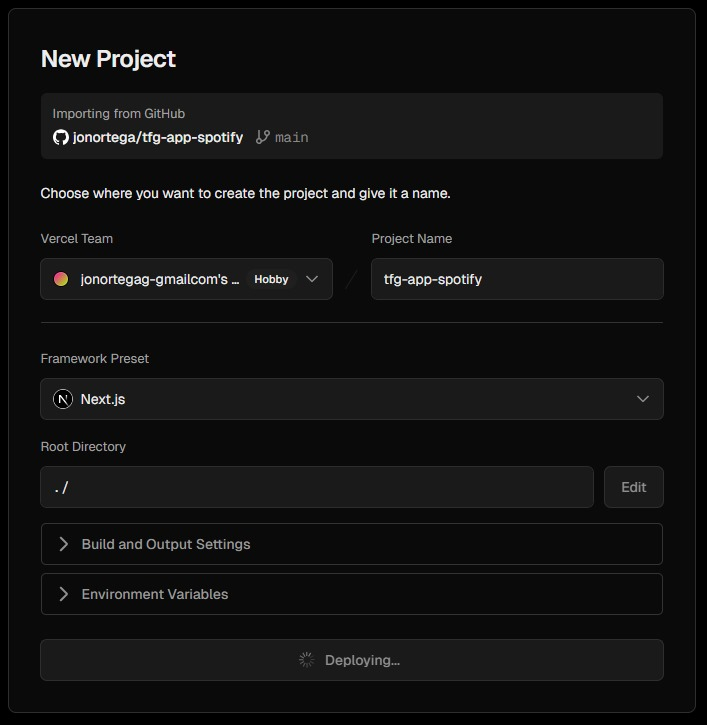
\includegraphics[width=0.5\textwidth]{figures/despliegue/creacion_proyecto.jpg}
    \caption{Pantalla de creación del proyecto tras conectarlo con el repositorio de \textit{GitHub}.}
    \label{fig:creacion_proyecto}
\end{figure}

Tras esperar a que se realice el buid correctamente, nuestra aplicación se encontrará en línea, con certificados SSL y con un dominio personal que \textit{Vercel} establecerá según el nombre del proyecto\footnote{Dominio del proyecto de este TFG: \href{https://tfg-app-spotify.vercel.app}{https://tfg-app-spotify.vercel.app}}. Existen dos diferentes entornos de despliegue:

\begin{itemize}
    \item \textit{Production}: Entorno principal, accesible para los usuarios finales desde el dominio establecido en la creación del proyecto. Se toma la rama \texttt{main} como la rama de producción.
    \item \textit{Preview}: Entorno de preproducción que se genera automáticamente al realizar cambios en cualquier rama distinta a la de producción (\texttt{main}). Se asigna un dominio único diferente a cada despliegue.
\end{itemize}

En nuestro caso, solo haremos uso del entorno \textit{production}. Cualquier cambio realizado en la rama \texttt{main} será detectado automáticamente por \textit{Vercel}, que creará un nuevo despliegue, realizará un nuevo build y actualizará la página en línea. En caso de que ocurra algún error, se revertirá automáticamente a la versión anterior del proyecto. Este proceso se realiza sin intervención manual, por lo que obtenemos un despliegue contínuo (CD) sin necesidad de configuraciones adicionales.

\subsection{Configuración de Variables de Entorno}

Para finalizar con la configuración del despliegue, es necesario agregar las variables de entorno en el panel de control de \textit{Vercel}. Cada entorno permite establecer variables específicas, pero en nuestro caso solo introduciremos, en el entorno de producción, las siguientes:

\begin{table}[htbp]
    \centering
    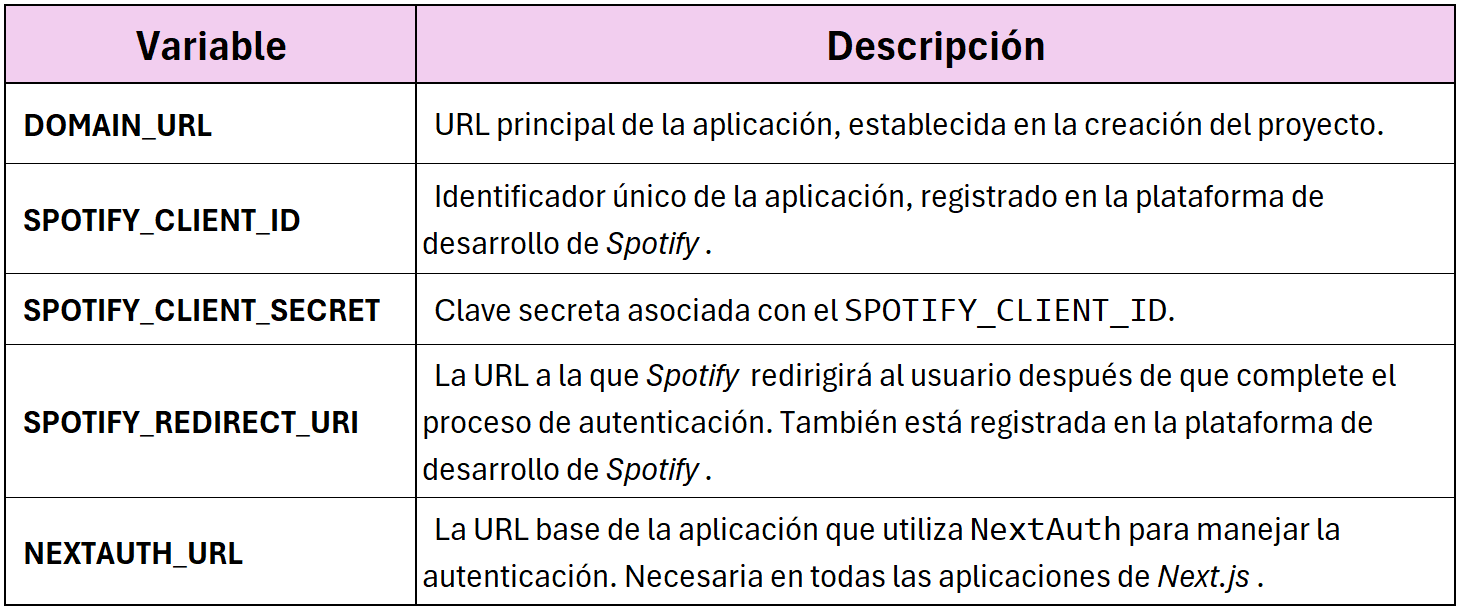
\includegraphics[width=0.9\textwidth]{figures/despliegue/variables_entorno.png}
    \captionsetup{skip=10pt}
    \caption{Variables de entorno necesarias en producción.}
    \label{tab:variables_entorno}
\end{table}

Es importante destacar que, para garantizar una transición fluida entre el entorno de desarrollo local y el de producción, se debe evitar codificar directamente las URLs en el código. En su lugar, se debe utilizar la variable de entorno \texttt{DOMAIN\_URL}, lo que permite que las URLs cambien automáticamente de \texttt{localhost} al dominio público correspondiente.

\subsection{Análisis y Monitoreo}

\textit{Vercel} ofrece un panel de control desde donde se pueden visualizar diversas métricas y modificar opciones de configuración. Para este proyecto, es importante monitorizar los indicadores de recursos consumidos (figura \ref{fig:usage_overview}), para asegurar que no llegan al límite del plan gratuito.

\begin{figure}[H]
    \centering
    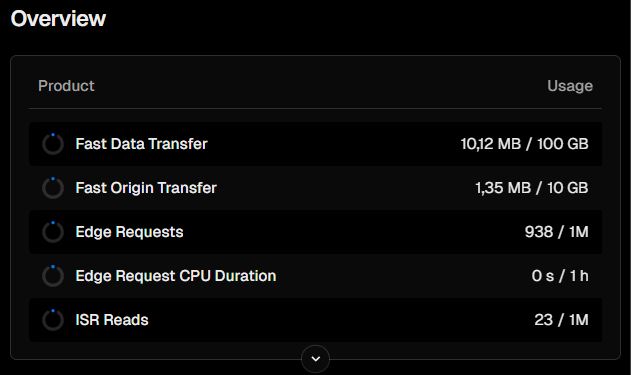
\includegraphics[width=0.6\textwidth]{figures/despliegue/usage_overview.png}
    \caption{Panel con la visión general de los recursos consumidos.}
    \label{fig:usage_overview}
\end{figure}

\newpage

Esto es especialmente relevante porque, en las plataformas de nube, se ha popularizado un ataque conocido como \textbf{Ataque de Agotamiento Económico} (\textit{Denial of Wallet} (DoW)) \cite{vercelDoW2025}. Son un tipo de ataque DoS, cuyo objetivo es consumir continuamente los recursos más ``pesados'', con el fin de obligar el escalado automático y agotar el presupuesto operativo de la aplicación. En el caso de este proyecto, al encontrarse dentro del plan gratuito, la consecuencia sería el consumo completo de los recursos disponibles; haciendo que \textit{Vercel} retirase la aplicación de producción, quedándose inoperativa hasta el siguiente ciclo mensual.

Por esta razón, \textit{Vercel} y otras plataformas similares ofrecen mecanismos de protección contra ataques DoS, permitiendo bloquear temporalmente este tipo de peticiones con el firewall integrado. Además, podemos acceder a ver los logs generados en el servidor durante la última hora y monitorizar el número de invocaciones, datos transferidos y peticiones por cada ruta de nuestra web.


% TODO: Comprobar si es posible hacer esto cuanto tenga los tests.
\section{Ejecución Automática de Tests}
Añadir al hacer el apartado de Pruebas.
% Una funcionalidad deseable en el despliegue es la ejecución automática de tests para garantizar que cada nueva versión sea estable antes de llegar a producción. Configurar GitHub Actions para ejecutar los tests antes de desplegar. Una posible estrategia es usar GitHub Actions para correr los tests unitarios y de integración antes de hacer el \textit{push} a la rama principal.
